% Autor szablonu: dr Roman Czapla
% Kompilacja: pdfLaTeX (dwukrotnie, aby zaktualizować spis treści).
% Wymagane logo uczelni: images/logo.png (ścieżka względem pliku głównego).
\documentclass[11pt,a4paper,oneside]{article}
\usepackage[utf8]{inputenc}
\usepackage[T1]{fontenc}
\usepackage[polish,provide=*]{babel}
\usepackage{lmodern,microtype}
\usepackage[margin=25mm,headheight=14pt]{geometry}
\usepackage{xcolor,graphicx,tabularx,booktabs,array,enumitem,fancyhdr,titlesec}
\usepackage[hidelinks]{hyperref}
\definecolor{accent}{HTML}{344B59}
\definecolor{hintcolor}{HTML}{58636A}
\hypersetup{pdfauthor={},pdftitle={Projekt inżynierski - Raport z realizacji projektu}}
\setlength{\parindent}{0pt}
\setlength{\parskip}{6pt}
\renewcommand{\arraystretch}{1.3}
\setlength{\emergencystretch}{2em}
\setlist[itemize]{leftmargin=*,itemsep=2pt,topsep=3pt}
\titleformat{\section}{\Large\bfseries\color{accent}}{\thesection.}{0.5em}{}
\titleformat{\subsection}{\large\bfseries\color{accent}}{\thesubsection.}{0.5em}{}
\pagestyle{fancy}
\fancyhf{}
\fancyhead[L]{\small Projekt inżynierski}
\fancyhead[R]{\small Raport z realizacji projektu}
\fancyfoot[C]{\small\thepage}
\renewcommand{\headrulewidth}{0.3pt}
\newcolumntype{Y}{>{\raggedright\arraybackslash}X}

% Podpowiedzi są widoczne podczas wypełniania szablonu.
% Przed oddaniem: uzupełnij pola, zastąp przykłady własną treścią
% i zmień poniższy przełącznik na \podpowiedzifalse.
\newif\ifpodpowiedzi
%\podpowiedzitrue
\podpowiedzifalse
\newcommand{\podpowiedz}[1]{\ifpodpowiedzi\par\begingroup\small\color{hintcolor}\textit{Wskazówka: #1}\par\endgroup\fi}
\newcommand{\pole}[1]{\textnormal{[#1]}}
% Znacznik miejsc do sprawdzenia przez zespół - przed oddaniem wyszukaj "\dopotw" i usuń wszystkie wystąpienia.
\newcommand{\dopotw}[1]{\textcolor{red}{\textbf{[DO POTWIERDZENIA: #1]}}}

% Dane dokumentu - uzupełnij w jednym miejscu.
% Ścieżkę logo można zmienić poniżej.
\newcommand{\pliklogo}{images/logo.png}
\newcommand{\logouczelni}{%
  \includegraphics[width=0.8\textwidth,height=40mm,keepaspectratio]{\pliklogo}%
}
\newcommand{\tytulprojektu}{Asystent bezpieczeństwa do monitorowania i~wykrywania anomalii w~środowisku chmurowym}
\newcommand{\rokakademicki}{{2026/2027}}
\newcommand{\semestrprojektu}{{zimowy}}
\newcommand{\numerRaportu}{{1}}
\newcommand{\okresOd}{{06.11.2026}}
\newcommand{\okresDo}{{20.11.2026}}
\newcommand{\datadokumentu}{{20.11.2026}}
\newcommand{\wersjadokumentu}{{1.0}}
\newcommand{\studentA}{{Karolina Graf}}
\newcommand{\studentB}{{Yuliia Lesyk}}
\newcommand{\studentC}{{Mylana Herasymenko}}
\newcommand{\albumA}{{171182}}
\newcommand{\albumB}{{168814}}
\newcommand{\albumC}{{168844}}
\newcommand{\prowadzacyA}{{dr Beata Krzaczek}}
\newcommand{\prowadzacyB}{{mgr Patryk Mazurek}}
% Adresy repozytoriów
\newcommand{\repokod}{https://github.com/hakalochka/Projekt-Inzynierski}
\newcommand{\repodok}{https://github.com/ytkodoshik/projekt_in-ynierski}
\newcommand{\zalaczniki}{https://github.com/ytkodoshik/projekt_in-ynierski/tree/main/Szablony_2026/raport_okresowy/images}

\begin{document}
\begin{titlepage}
\centering
{\large Uniwersytet Komisji Edukacji Narodowej w Krakowie\par}
{\normalsize Instytut Bezpieczeństwa i Informatyki\par}
\vspace{8mm}
\logouczelni\par
\vspace{10mm}
{\Large\bfseries\color{accent} PROJEKT INŻYNIERSKI\par}
\vspace{3mm}
{\large Raport z realizacji projektu\par}
\vspace{3mm}
Raport nr \numerRaportu\par
Okres: \okresOd{} - \okresDo\par
\vspace{15mm}
{\LARGE\bfseries\tytulprojektu\par}
\vspace{15mm}
{\small ZESPÓŁ PROJEKTOWY\par}
\vspace{3mm}
\begin{tabular}{ll}
\studentA & Nr albumu: \albumA\\
\studentB & Nr albumu: \albumB\\
\studentC & Nr albumu: \albumC
\end{tabular}
\vspace{12mm}

{\small PROWADZĄCY ZAJĘCIA PROJEKTOWE\par}
\vspace{3mm}
\prowadzacyA\par
\prowadzacyB\par
\vfill
Rok akademicki: \rokakademicki\quad Semestr: \semestrprojektu\par
Data dokumentu: \datadokumentu\quad Wersja: \wersjadokumentu\par
\vspace{6mm}
Kraków\par

\end{titlepage}

\tableofcontents
\podpowiedz{Przygotuj jeden wspólny raport zespołu za okres między poprzednim a bieżącym spotkaniem. Pierwszy raport jest wymagany na trzecie spotkanie i obejmuje prace między drugim a trzecim spotkaniem. Opisuj wyłącznie prace z podanego okresu, rozróżniając zadania zakończone i będące w toku. Uzupełnij pola, usuń przykłady i wyłącz podpowiedzi przed oddaniem.}

\section{Postępy prac nad projektem}
\subsection{Zespół projektowy}
\podpowiedz{Podaj aktualne dane kontaktowe wszystkich członków zespołu. Imiona i nazwiska powinny być zgodne ze stroną tytułową. W przypadku zespołu dwuosobowego zatwierdzonego przez dyrekcję instytutu usuń dane trzeciej osoby ze strony tytułowej, obu tabel oraz odpowiedni blok opisu prac.}
\begin{tabularx}{\textwidth}{@{}Y p{0.22\textwidth} Y@{}}
\toprule
Imię i nazwisko & Numer albumu & E-mail\\
\midrule
\studentA & \albumA & {s171182@student.uken.krakow.pl}\\
\studentB & \albumB & {s168814@student.uken.krakow.pl}\\
\studentC & \albumC & {s168844@student.uken.krakow.pl}\\
\bottomrule
\end{tabularx}

\subsection{Zestawienie zadań}
\podpowiedz{Dla każdej osoby wymień zadania z danego okresu i ich stan: zakończone, w toku lub zablokowane. Przy pracy wspólnej wskaż konkretny wkład każdej osoby. Odwołania do opisów generuj poleceniem \texttt{\textbackslash ref}; nie wpisuj ręcznie numerów sekcji. Powielaj wiersze i opisy według potrzeb.}
W okresie sprawozdawczym zamknięto etap~1 harmonogramu (środowisko chmurowe i~system SIEM) i~rozpoczęto etap~2 (przygotowanie danych i~modeli uczenia maszynowego). Punktem wyjścia była instancja EC2 \textit{Serwer-SIEM} utworzona 05.11.2026, tuż przed rozpoczęciem okresu.

\begin{tabularx}{\textwidth}{@{}p{0.20\textwidth} Y p{0.15\textwidth} p{0.08\textwidth}@{}}
\toprule
Osoba & Zadanie & Stan & Opis\\
\midrule
\studentA & Pozyskanie i~wstępna analiza zbioru CICIDS2017, notatnik \texttt{prepare\_data.ipynb} \dopotw{osoba} & w toku & \ref{zadanie-a}\\
\studentB & Dokończenie konfiguracji Wazuh i~zabezpieczenie środowiska AWS & zakończone & \ref{zadanie-b1}\\
\studentB & Wdrożenie agenta Wazuh i~test wykrywania ataku brute force & zakończone & \ref{zadanie-b2}\\
\studentB & Repozytorium dokumentacji i~przygotowanie materiałów do raportu & zakończone & \ref{zadanie-b3}\\
\studentC & Instalacja Wazuh, konta użytkowników Linux, dostęp SSH, środowisko VS Code i~repozytorium kodu \dopotw{osoba} & zakończone & \ref{zadanie-c}\\
\bottomrule
\end{tabularx}

\newpage
\subsection{Opis wykonanych prac}
\podpowiedz{Dla każdego zadania podaj cel, wykonane czynności, konkretny rezultat i sposób jego sprawdzenia. Wskaż materiały potwierdzające prace, np. pliki, commity, zgłoszenia, zrzuty ekranu lub załączniki. Przy zadaniu w toku opisz, co już wykonano i co pozostało. Jeśli dana osoba nie wykonała prac w tym okresie, wskaż to wprost i wyjaśnij przyczynę.}

\subsubsection{\studentA: Pozyskanie i~wstępna analiza zbioru CICIDS2017}\label{zadanie-a}
\dopotw{przypisanie zadania do osoby i~szczegóły wykonania}\par
\textbf{Cel i zakres:} przygotowanie danych uczących do modeli wykrywania anomalii w~ruchu sieciowym, zgodnie z~założeniem projektu o~wykorzystaniu publicznych zbiorów danych.\par
\textbf{Wykonane prace:} pobrano zbiór CICIDS2017 (Intrusion Detection Evaluation Dataset, Canadian Institute for Cybersecurity) za pomocą biblioteki \texttt{kagglehub}. Przygotowano notatnik \texttt{scr/prepare\_data.ipynb}, który wczytuje 8~plików CSV z~katalogu \texttt{MachineLearningCVE} (ruch z~5~dni roboczych, m.in. pliki z~atakami PortScan, DDoS, DoS i~SSH/FTP-Patator) i~łączy je w~jedną ramkę danych (rys.~\ref{fig:dane}). Wykonano wstępny przegląd struktury danych: typy kolumn, braki danych, zajętość pamięci. Do repozytorium dodano plik \texttt{requirements.txt} z~wymaganymi bibliotekami. Dane nie są przechowywane w~repozytorium ze względu na rozmiar (ponad 1~GB) i~są wykluczone w~\texttt{.gitignore}.\par
\textbf{Rezultat i weryfikacja:} połączony zbiór zawiera 2\,830\,743 rekordy i~79~kolumn (78~cech przepływów sieciowych wygenerowanych narzędziem CICFlowMeter oraz etykieta \texttt{Label}), co zajmuje ok.~1,7~GB pamięci. Zadanie jest w~toku. Pozostało oczyszczenie danych (nazwy kolumn ze spacjami, wartości nieskończone, duplikaty, kolumny stałe), wybór klas odpowiadających planowanym symulacjom ataków (BENIGN, PortScan, SSH-Patator) oraz stratyfikowany podział na zbiór treningowy i~testowy ze skalowaniem dopasowanym wyłącznie na zbiorze treningowym.\par
\textbf{Materiały potwierdzające:} Z15, Z16; notatnik \texttt{scr/prepare\_data.ipynb} w~repozytorium kodu (gałąź \texttt{model-training}).

\begin{figure}[htbp]
\centering
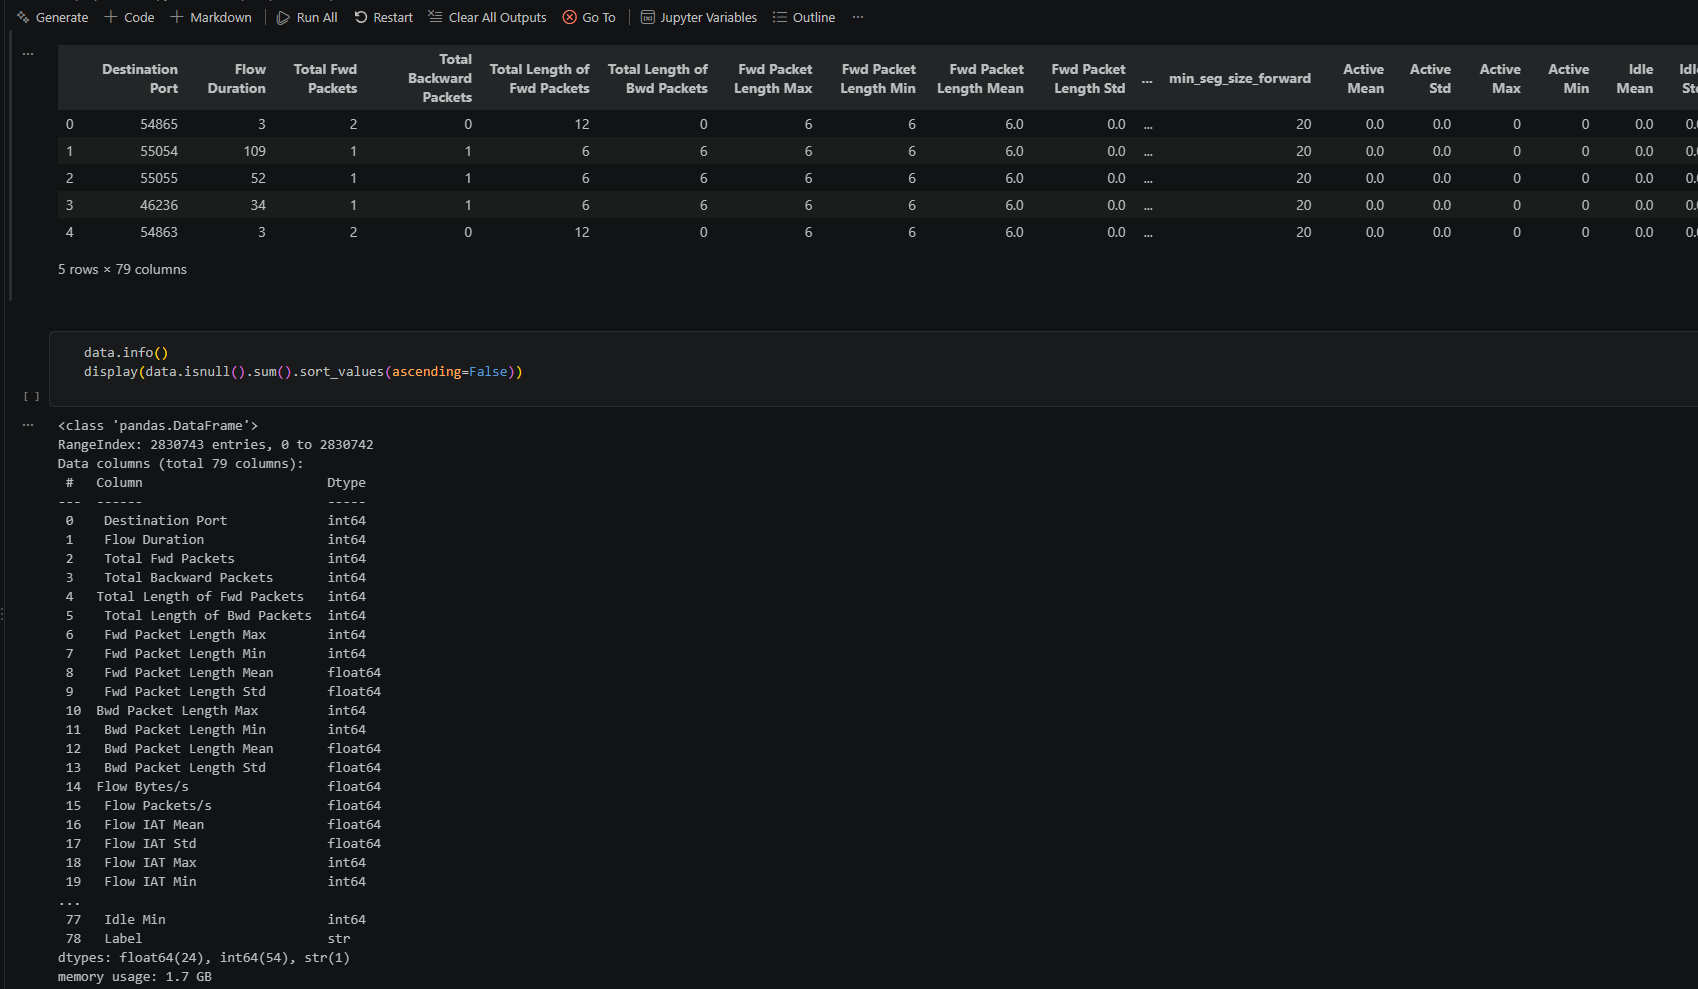
\includegraphics[width=0.85\textwidth]{images/Z16_cicids_struktura_danych.png}
\caption{Wczytany zbiór CICIDS2017: podgląd danych i~struktura kolumn (2\,830\,743 rekordy, 79 kolumn).}
\label{fig:dane}
\end{figure}

\subsubsection{\studentB: Dokończenie konfiguracji Wazuh i~zabezpieczenie środowiska AWS}\label{zadanie-b1}
\textbf{Cel i zakres:} zamknięcie etapu~1 harmonogramu: sprawdzenie działania systemu SIEM, dostosowanie zasobów serwera do wymagań Wazuh oraz ograniczenie dostępu do serwera z~internetu.\par
\textbf{Wykonane prace:}
\begin{itemize}
\item Sprawdzono działanie trzech komponentów Wazuh 4.14.10 (manager, indexer, dashboard) poleceniem \texttt{systemctl status}. Panel Wazuh Dashboard jest dostępny przez HTTPS.
\item Instancja t3.medium ma 4~GB RAM, a~wolna pamięć wynosiła ok.~1,3~GB przy braku pamięci wymiany. Dodano 4~GB pamięci wymiany (\texttt{/swapfile}) z~trwałym wpisem w~\texttt{/etc/fstab}.
\item Zajętość dysku wynosiła 84\%, a~indeks Wazuh (OpenSearch) przy przekroczeniu progów zapełnienia przestaje przyjmować nowe dane. Wolumen EBS powiększono z~30 do 50~GiB bez zatrzymywania serwera; zajętość spadła do 49\%.
\item W~grupie zabezpieczeń serwera (\texttt{launch-wizard-1}) usunięto domyślne reguły zezwalające na dostęp SSH (22) i~HTTPS (443) z~dowolnego adresu (\texttt{0.0.0.0/0}). Dostęp ograniczono do adresów IP członkiń zespołu, po jednej regule na osobę z~opisem. Porty agenta Wazuh (1514 -- przesyłanie zdarzeń, 1515 -- rejestracja) otwarto wyłącznie dla grupy zabezpieczeń instancji monitorowanej (\texttt{agent-sg}), a~nie dla adresów IP (rys.~\ref{fig:sg}).
\end{itemize}
\textbf{Rezultat i weryfikacja:} wszystkie usługi Wazuh mają status \textit{active (running)}, a~status managera w~panelu potwierdza działanie kluczowych procesów (\texttt{analysisd}, \texttt{remoted}, \texttt{authd}, \texttt{logcollector}). Polecenia \texttt{free -h} i~\texttt{df -h} potwierdziły dostępność 4~GB pamięci wymiany i~25~GB wolnego miejsca na dysku. Konsola AWS przestała wyświetlać ostrzeżenie o~regułach otwartych dla wszystkich adresów.\par
\textbf{Materiały potwierdzające:} Z01, Z02, Z03, Z04.

\begin{figure}[htbp]
\centering
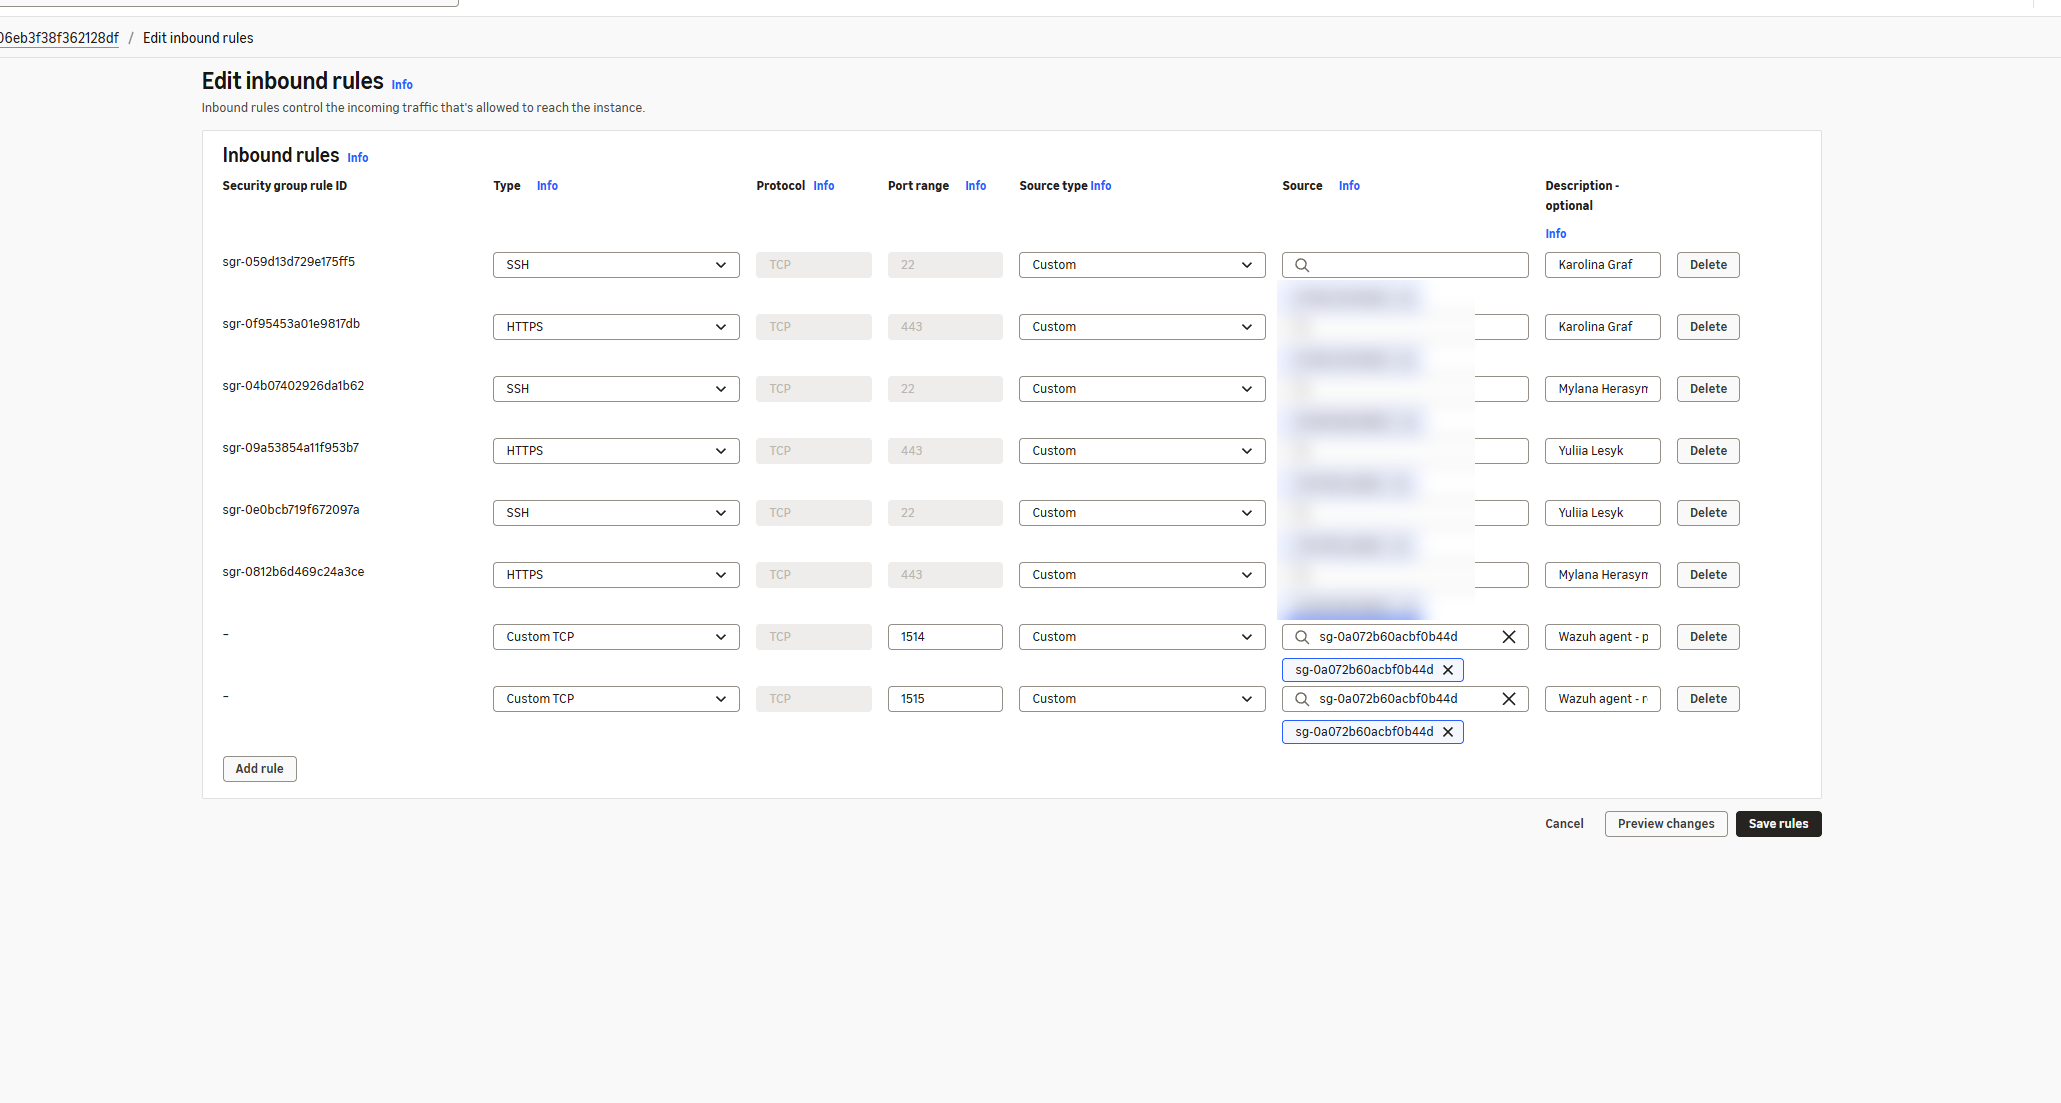
\includegraphics[width=0.9\textwidth]{images/Z02_security_group_po.png}
\caption{Reguły ruchu przychodzącego serwera SIEM po zmianach: SSH i~HTTPS tylko z~adresów zespołu (zamazane), porty 1514/1515 tylko dla grupy \texttt{agent-sg}.}
\label{fig:sg}
\end{figure}

\subsubsection{\studentB: Wdrożenie agenta Wazuh i~test wykrywania ataku brute force}\label{zadanie-b2}
\textbf{Cel i zakres:} podłączenie monitorowanego hosta do systemu SIEM i~sprawdzenie, czy cały łańcuch zbierania logów i~generowania alertów działa na przykładzie symulowanego ataku.\par
\textbf{Wykonane prace:}
\begin{itemize}
\item Uruchomiono drugą instancję EC2 \textit{Agent-ofiara} (Ubuntu Server 24.04 LTS, t3.micro) w~tej samej sieci VPC co serwer, z~osobną grupą zabezpieczeń \texttt{agent-sg} i~dostępem SSH tylko z~adresów zespołu (rys.~\ref{fig:instancje}).
\item Zainstalowano agenta Wazuh 4.14.10 (zgodnego z~wersją managera) według kreatora \textit{Deploy new agent}. Agent łączy się z~serwerem przez prywatny adres IP w~VPC, więc ruch między nimi nie przechodzi przez publiczny internet.
\item Przeprowadzono symulację ataku brute force: z~komputera członkini zespołu wykonano serię 10~prób logowania SSH na nieistniejące konto \texttt{hacker}.
\end{itemize}
\textbf{Rezultat i weryfikacja:} agent zarejestrował się pod identyfikatorem 001 i~ma status \textit{active} (rys.~\ref{fig:agent}). Po podłączeniu agenta liczba alertów w~panelu wzrosła z~58 do 343, głównie w~wyniku automatycznej oceny konfiguracji (SCA) i~monitorowania integralności plików na nowym hoście. Podczas symulacji ataku system w~ciągu kilku sekund wygenerował 20~zdarzeń: alerty reguły 5710 (poziom~5) dla pojedynczych prób logowania oraz alert reguły 5712 (poziom~10), który klasyfikuje serię prób jako atak brute force (rys.~\ref{fig:alerty}). Reguła 5712 jest uruchamiana po co najmniej 8~nieudanych próbach z~jednego adresu (\texttt{rule.frequency}). Alert został automatycznie wzbogacony o~geolokalizację adresu źródłowego oraz mapowanie na MITRE ATT\&CK: technika T1110 Brute Force, taktyka Credential Access (rys.~\ref{fig:alert5712}). Test potwierdził poprawne działanie łańcucha: zdarzenie na hoście $\rightarrow$ agent $\rightarrow$ manager $\rightarrow$ indexer $\rightarrow$ dashboard.\par
\textbf{Materiały potwierdzające:} Z05--Z14.

\begin{figure}[htbp]
\centering
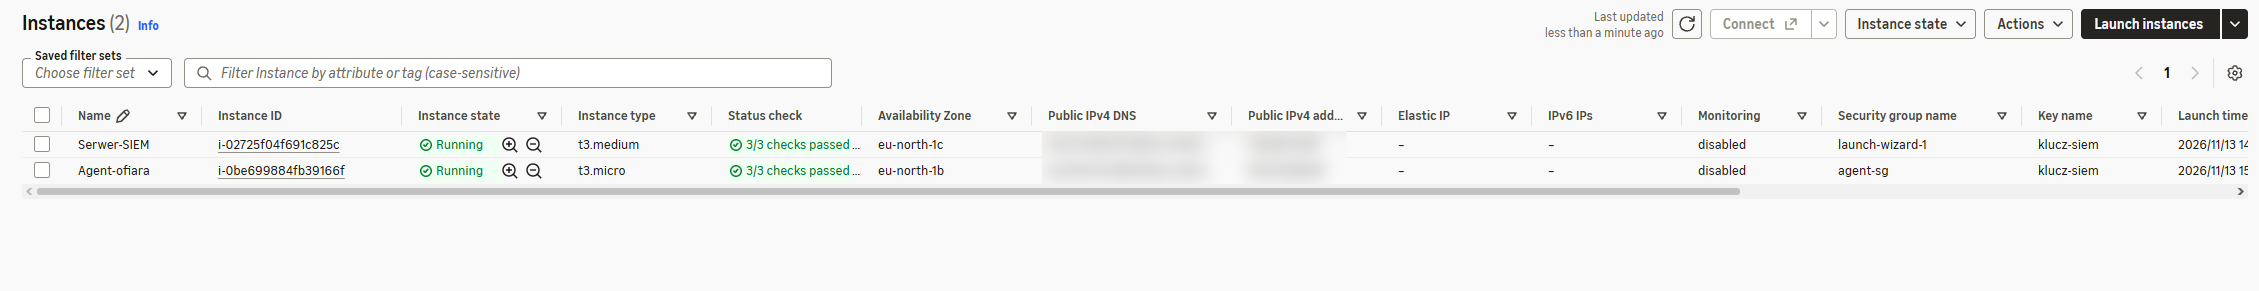
\includegraphics[width=\textwidth]{images/Z07_instancje_ec2.png}
\caption{Instancje EC2 projektu: serwer SIEM (t3.medium) i~instancja monitorowana z~agentem Wazuh (t3.micro). Adresy publiczne zamazano.}
\label{fig:instancje}
\end{figure}

\begin{figure}[htbp]
\centering
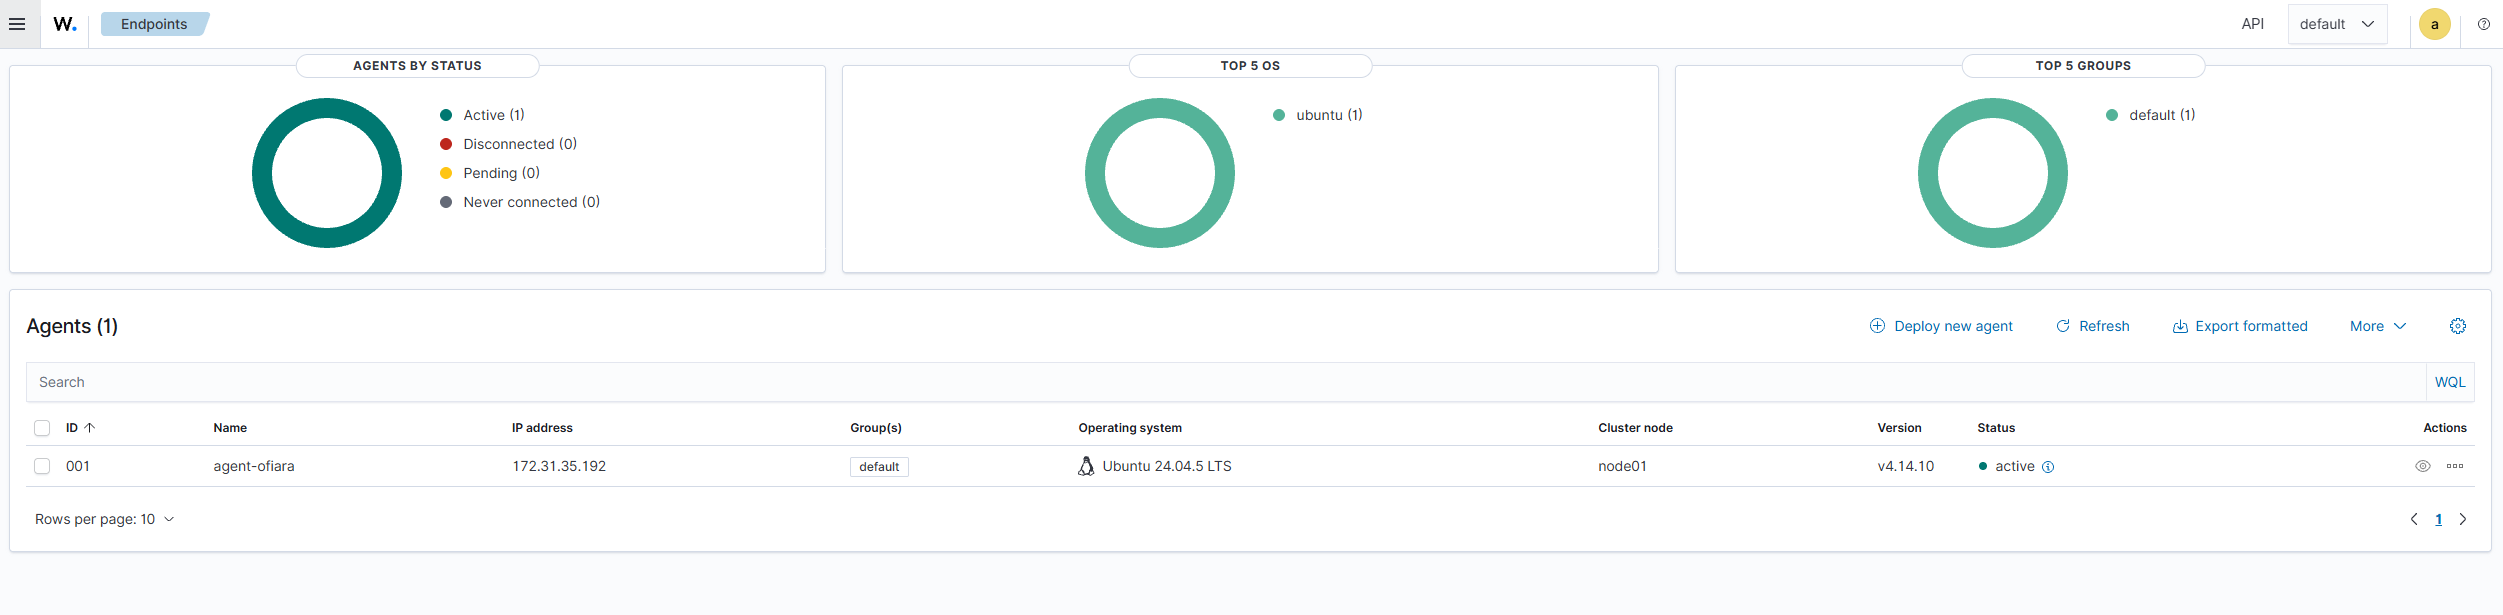
\includegraphics[width=\textwidth]{images/Z09_wazuh_endpoints_agent.png}
\caption{Lista agentów w~Wazuh Dashboard: agent na instancji monitorowanej (Ubuntu 24.04.5 LTS, v4.14.10) ze statusem aktywnym.}
\label{fig:agent}
\end{figure}

\begin{figure}[htbp]
\centering
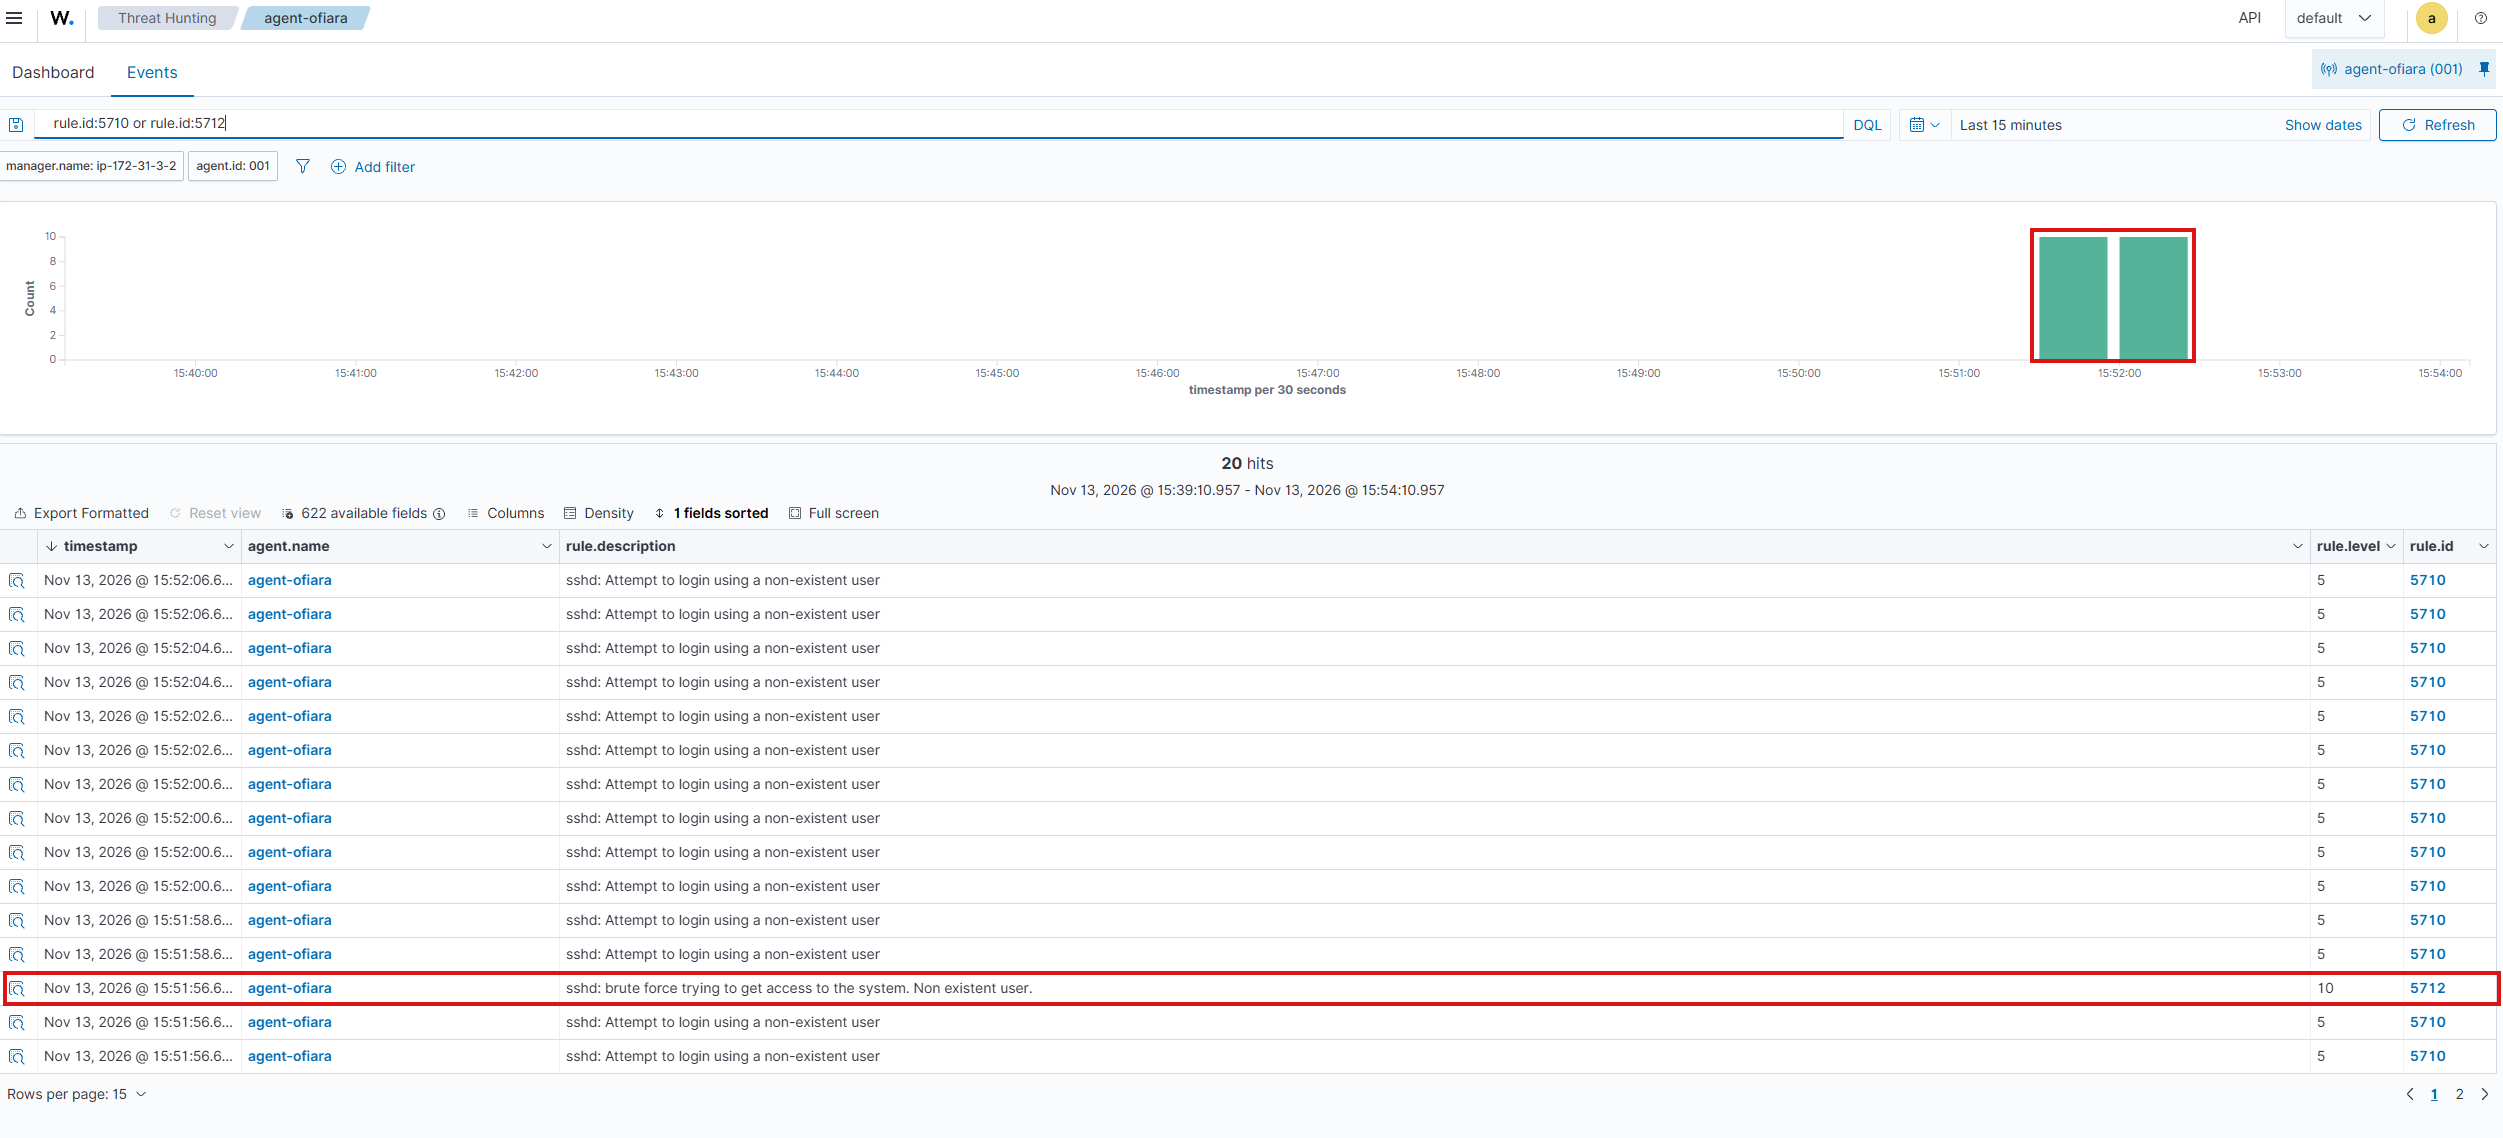
\includegraphics[width=\textwidth]{images/Z12_alerty_brute_force.png}
\caption{Alerty wygenerowane podczas symulowanego ataku brute force SSH. Zaznaczono wzrost liczby zdarzeń w~chwili ataku oraz alert reguły 5712 (poziom 10).}
\label{fig:alerty}
\end{figure}

\begin{figure}[htbp]
\centering
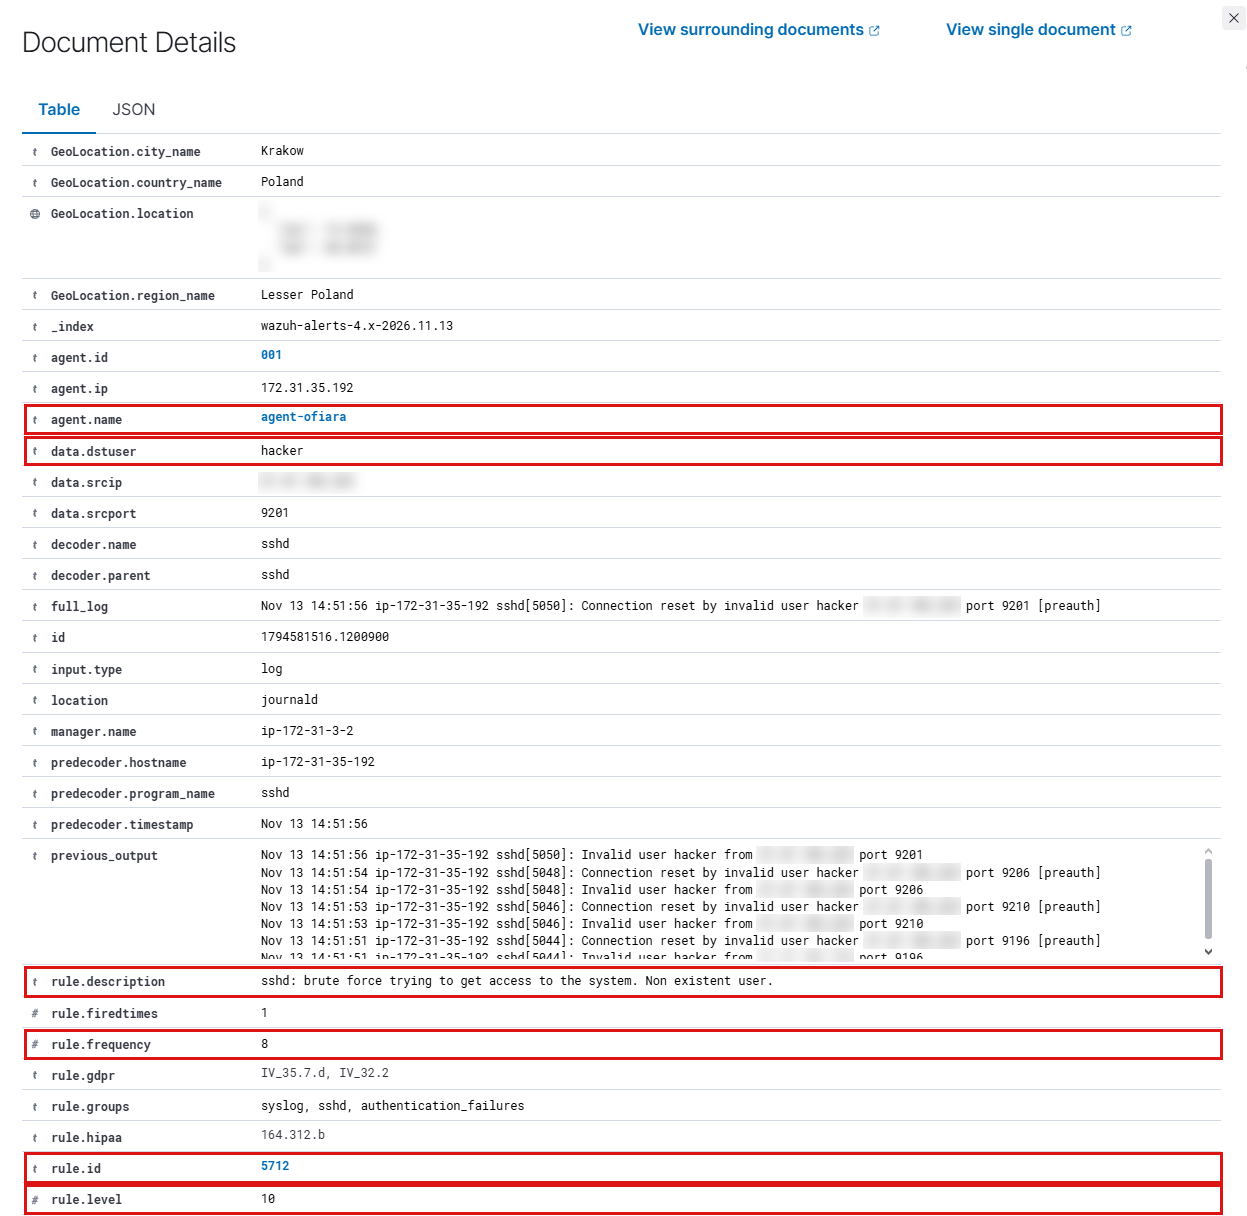
\includegraphics[width=0.75\textwidth]{images/Z13_alert_5712_szczegoly.png}
\caption{Szczegóły alertu 5712: zaatakowany host, użyta nazwa konta, opis i~poziom reguły oraz próg korelacji (\texttt{rule.frequency}~=~8). Adres IP i~współrzędne geolokalizacji zamazano.}
\label{fig:alert5712}
\end{figure}

\subsubsection{\studentB: Repozytorium dokumentacji i~przygotowanie materiałów do raportu}\label{zadanie-b3}
\dopotw{czy repozytorium dokumentacji powstało w~tym okresie}\par
\textbf{Cel i zakres:} zgromadzenie materiałów potwierdzających wykonane prace w~sposób bezpieczny do publikacji w~publicznym repozytorium.\par
\textbf{Wykonane prace:} przygotowano zrzuty ekranu dokumentujące konfigurację środowiska i~wyniki testów. Na zrzutach zamazano publiczne adresy IP instancji, domowe adresy IP członkiń zespołu, identyfikator konta AWS i~współrzędne geolokalizacji. Materiały umieszczono w~repozytorium dokumentacji (\texttt{raporty/raport1/zalaczniki/}).\par
\textbf{Rezultat i weryfikacja:} 17~opisanych załączników (Z01--Z16) w~repozytorium dokumentacji. Każdy zrzut przejrzano pod kątem danych wrażliwych przed publikacją.\par
\textbf{Materiały potwierdzające:} \url{\zalaczniki}.

\subsubsection{\studentC: Instalacja Wazuh, konta użytkowników i~środowisko pracy}\label{zadanie-c}
\dopotw{przypisanie zadania do osoby, daty wykonania i~szczegóły}\par
\textbf{Cel i zakres:} przygotowanie wspólnego środowiska pracy zespołu na serwerze chmurowym i~lokalnie.\par
\textbf{Wykonane prace:} zainstalowano Wazuh w~wariancie \textit{all-in-one} (manager, indexer i~dashboard na jednej instancji). Skonfigurowano dostęp do serwera przez SSH z~uwierzytelnianiem kluczem. Utworzono osobne konta użytkowników systemu Linux dla każdej członkini zespołu, co zapewnia rozliczalność działań i~pozwala nie współdzielić konta \texttt{ubuntu}. Środowisko pracy z~kodem zmieniono z~Google Colab na Visual Studio Code. Utworzono repozytorium kodu z~katalogiem \texttt{scr/}, w~którym przygotowano szkielet notatników (\texttt{download\_dataset}, \texttt{prepare\_data}, \texttt{preprocess}, \texttt{train}, \texttt{evaluate}), oraz gałąź roboczą \texttt{model-training}.\par
\textbf{Rezultat i weryfikacja:} wszystkie członkinie zespołu mogą zalogować się na serwer na własne konta. Panel Wazuh był dostępny przed dalszą konfiguracją opisaną w~pkt~\ref{zadanie-b1}.\par
\textbf{Materiały potwierdzające:} Z04, Z05; repozytorium kodu \url{\repokod}.

\subsection{Problemy i zmiany w planie}
\podpowiedz{Wskaż trudności, przyczyny opóźnień, wpływ na harmonogram oraz podjęte lub proponowane działania. Odnotuj istotne zmiany zakresu uzgodnione z prowadzącymi. Jeśli nie wystąpiły problemy ani zmiany, napisz to wprost.}
\begin{itemize}
\item \textbf{Niewystarczające zasoby serwera.} Wazuh w~wariancie \textit{all-in-one} zalecany jest dla maszyn z~co najmniej 8~GB RAM, a~instancja t3.medium ma 4~GB. Dysk był zapełniony w~84\%. Problem rozwiązano przez dodanie pamięci wymiany i~powiększenie wolumenu (pkt~\ref{zadanie-b1}). Jeśli przy większej liczbie zdarzeń wystąpią spadki wydajności, typ instancji zostanie zmieniony na t3.large bez reinstalacji systemu.
\item \textbf{Domyślnie otwarty dostęp do serwera.} Kreator EC2 utworzył reguły SSH i~HTTPS dostępne z~dowolnego adresu. Zostały one zastąpione regułami ograniczonymi do adresów zespołu. Wadą tego rozwiązania jest konieczność aktualizacji reguł przy zmianie adresu IP. Jako alternatywę rozważamy AWS Systems Manager Session Manager.
\item \textbf{Niespójne środowisko Python.} Biblioteki były instalowane do innej wersji interpretera (3.14) niż używana przez notatnik (3.13), a~zbiór danych nie znajduje się w~repozytorium, więc ścieżki do danych nie działały na wszystkich komputerach. Zespół ustala wspólną wersję Pythona, uzupełnia \texttt{requirements.txt} o~\texttt{kagglehub} i~wczytuje dane przez \texttt{kagglehub.dataset\_download}, co zapewnia tę samą ścieżkę na każdym komputerze.
\item \textbf{Niezgodność cech danych uczących z~logami Wazuh.} Zbiór CICIDS2017 opisuje przepływy sieciowe (cechy z~CICFlowMeter), których nie zawierają logi zbierane przez Wazuh. Planujemy wygenerować te same cechy z~ruchu przechwyconego na instancji monitorowanej (\texttt{tcpdump} + \texttt{cicflowmeter}). Pozwoli to wykrywać ataki niewidoczne w~logach systemowych, np. skanowanie portów. Wyniki modelu będą zapisywane do pliku logu odczytywanego przez agenta Wazuh. Wykonalność podejścia sprawdzimy na początku kolejnego okresu. W~razie niepowodzenia model zostanie zbudowany na cechach wyliczanych z~alertów Wazuh, np. liczbie nieudanych logowań z~jednego adresu w~oknie czasowym.
\item \textbf{Harmonogram.} Etap~1 planowano zakończyć 07.11.2026. Konfigurację Wazuh zakończono 13.11.2026, a~przesunięcie nie wpływa na termin etapu~2 (08.12.2026). Zmiana środowiska z~Google Colab na Visual Studio Code nie zmienia zakresu projektu.
\end{itemize}

\subsection{Plan prac na kolejny okres}
\podpowiedz{Wymień zadania do kolejnego spotkania, osoby odpowiedzialne oraz oczekiwane rezultaty. Uwzględnij zadania niezakończone i zależności między pracami.}
\dopotw{przypisanie osób}

\begin{tabularx}{\textwidth}{@{}Y p{0.25\textwidth} Y@{}}
\toprule
Zadanie & Odpowiedzialni & Oczekiwany rezultat\\
\midrule
Oczyszczenie danych CICIDS2017, wybór klas, podział train/test i~skalowanie & \studentA & Zapisane zbiory treningowy i~testowy oraz skaler, statystyki przed i~po czyszczeniu\\
Test wykonalności: przechwycenie ruchu (\texttt{tcpdump}) podczas skanowania \texttt{nmap}, konwersja \texttt{cicflowmeter}, porównanie cech z~CICIDS2017 & \studentB & Decyzja o~sposobie integracji modelu ML z~Wazuh\\
Pierwsze modele: Random Forest (nadzorowany) i~Isolation Forest (nienadzorowany) & \studentA, \studentC & Metryki precision, recall, F1, FPR i~macierz pomyłek na zbiorze testowym\\
Wybór i~przeniesienie reguł Sigma (brute force SSH, skanowanie portów) do formatu reguł Wazuh & \studentC & Reguły XML wdrożone na serwerze i~przetestowane\\
Aktualizacja dokumentacji projektu (technologie, sekcja materiałów końcowych, wersja Pythona) & wszystkie & Dokument w~wersji 1.2\\
\bottomrule
\end{tabularx}

\subsection{Wykorzystanie AI i materiałów zewnętrznych}
\podpowiedz{Jeżeli AI miała istotny wpływ na prace z tego okresu, wskaż narzędzie, zadania, zakres zastosowania oraz sposób weryfikacji wyników. Rozróżnij wsparcie prac od rozwijania funkcji AI będących częścią projektu. Nie dołączaj pełnej historii rozmów ani wszystkich promptów. Możesz odwołać się do opisów zadań zamiast powtarzać informacje. Gdy nie korzystano z AI, wpisz tę informację.}
\textbf{AI:} w~zadaniach opisanych w~pkt~\ref{zadanie-b1}--\ref{zadanie-b3} korzystano z~asystenta Claude (Anthropic) jako wsparcia prac. Asystent pomagał w~rozpisaniu kolejnych kroków konfiguracji AWS i~Wazuh (grupy zabezpieczeń, pamięć wymiany, powiększenie dysku, instalacja agenta, scenariusz testu brute force), w~diagnozie błędów środowiska Python w~notatniku, w~propozycji kodu do czyszczenia i~podziału danych oraz w~zamazaniu danych wrażliwych na zrzutach ekranu. Każdy krok weryfikowano: sprawdzano status usług, wynik poleceń systemowych i~widok w~konsoli AWS, a~poprawność całej konfiguracji potwierdził test wykrywania ataku. Funkcje AI będące częścią projektu (modele ML wykrywające anomalie) nie zostały jeszcze zaimplementowane. \dopotw{czy pozostałe osoby korzystały z~innych narzędzi AI}\par
\podpowiedz{Wskaż nowe źródła, biblioteki, modele, dane, zasoby lub cudze fragmenty kodu wykorzystane w tym okresie oraz ich pochodzenie i warunki wykorzystania. W razie potrzeby dodaj wykaz źródeł z odnośnikami.}
\textbf{Materiały zewnętrzne:}
\begin{itemize}
\item Wazuh 4.14.10 (manager, indexer, dashboard, agent): oprogramowanie open source na licencji GPLv2, \url{https://documentation.wazuh.com}. Wykorzystano wbudowane reguły detekcji 5710 i~5712.
\item Zbiór CICIDS2017, Canadian Institute for Cybersecurity, University of New Brunswick, \url{https://www.unb.ca/cic/datasets/ids-2017.html}, pobrany z~kopii w~serwisie Kaggle (\texttt{mdalamintalukder/cicids2017}). Wykorzystanie zgodnie z~warunkami CIC wymaga cytowania pracy: I.~Sharafaldin, A.~H.~Lashkari, A.~A.~Ghorbani, \textit{Toward Generating a~New Intrusion Detection Dataset and Intrusion Traffic Characterization}, ICISSP 2018.
\item Biblioteki Python: pandas, NumPy, scikit-learn, matplotlib (licencje BSD), seaborn, joblib (BSD), kagglehub (Apache 2.0).
\item Infrastruktura: Amazon EC2 (region eu-north-1), obraz Ubuntu Server 24.04 LTS (Canonical).
\end{itemize}

\subsection{Załączniki i aktualna wersja projektu}

\podpowiedz{Podaj adres repozytorium lub uzgodnionego z prowadzącymi miejsca przechowywania materiałów. W polu „Wersja na koniec okresu” wskaż stan projektu opisany w raporcie: identyfikator commitu, tag albo nazwę i datę wersji plików, np. animacja-v03-2026-10-25. Nie chodzi tu o wersję dokumentu raportu. W tabeli wymień materiały potwierdzające wykonane prace, np. wyniki testów, zrzuty ekranu, pliki projektu lub próbne rendery. W kolumnie „Oznaczenie” nadaj im kolejne symbole Z1, Z2 itd.; w kolumnie „Plik / odnośnik” podaj nazwę pliku lub adres umożliwiający dostęp; w kolumnie „Opis i powiązane zadanie” wyjaśnij, co materiał przedstawia i którego zadania dotyczy, np. „Wyniki testów logowania opisanych w pkt 1.3.1”. Do oznaczeń załączników odwołuj się w opisach wykonanych prac. Dodaj lub usuń wiersze według potrzeb. Sam odnośnik do materiałów nie zastępuje opisu prac w raporcie.}

\textbf{Repozytorium lub miejsce przechowywania materiałów:}\\
kod projektu: \url{\repokod}\\
dokumentacja i~załączniki: \url{\repodok}\\
załączniki do raportu: \url{\zalaczniki}\par

\textbf{Wersja na koniec okresu:}\\
repozytorium kodu, gałąź \texttt{model-training}, tag \texttt{raport1-2026-11-20}\\ \dopotw{utworzyć tag lub wpisać identyfikator commitu}\par

\begin{tabularx}{\textwidth}{@{}p{0.12\textwidth} >{\footnotesize\raggedright\arraybackslash}p{0.37\textwidth} Y@{}}
\toprule
Oznaczenie & Plik / odnośnik & Opis i powiązane zadanie\\
\midrule
Z01 & \texttt{Z01\_security\_group\_przed.png} & Domyślne reguły grupy zabezpieczeń serwera (\texttt{0.0.0.0/0}) przed zmianą, pkt~\ref{zadanie-b1}\\
Z02 & \texttt{Z02\_security\_group\_po.png} & Reguły po ograniczeniu dostępu i~otwarciu portów agenta, pkt~\ref{zadanie-b1}\\
Z03 & \texttt{Z03\_wolumen\_50GiB.png} & Wolumen EBS serwera po powiększeniu do 50~GiB, pkt~\ref{zadanie-b1}\\
Z04 & \texttt{Z04\_wazuh\_status\_managera.png} & Status usług managera Wazuh 4.14.10, pkt~\ref{zadanie-c} i~\ref{zadanie-b1}\\
Z05 & \texttt{Z05\_wazuh\_overview\_przed\_agentem.png} & Panel Wazuh przed podłączeniem agenta, pkt~\ref{zadanie-b2}\\
Z06 & \texttt{Z06a\_ofiara\_ami\_typ.png},\newline \texttt{Z06b\_ofiara\_siec\_agent\_sg.png} & Konfiguracja instancji monitorowanej (obraz, typ, sieć, grupa \texttt{agent-sg}), pkt~\ref{zadanie-b2}\\
Z07 & \texttt{Z07\_instancje\_ec2.png} & Obie instancje EC2 w~stanie \textit{Running}, pkt~\ref{zadanie-b2}\\
Z08 & \texttt{Z08\_status\_agenta.png} & Usługa \texttt{wazuh-agent} na instancji monitorowanej, pkt~\ref{zadanie-b2}\\
Z09 & \texttt{Z09\_wazuh\_endpoints\_agent.png} & Agent 001 ze statusem aktywnym w~panelu, pkt~\ref{zadanie-b2}\\
Z10 & \texttt{Z10\_wazuh\_overview\_agent\_aktywny.png} & Panel główny po podłączeniu agenta, pkt~\ref{zadanie-b2}\\
Z11 & \texttt{Z11\_symulacja\_brute\_force.png} & Seria prób logowania SSH (symulacja ataku), pkt~\ref{zadanie-b2}\\
Z12 & \texttt{Z12\_alerty\_brute\_force.png} & Alerty 5710 i~5712 wygenerowane podczas ataku, pkt~\ref{zadanie-b2}\\
Z13 & \texttt{Z13\_alert\_5712\_szczegoly.png} & Szczegóły alertu 5712 i~korelacja zdarzeń, pkt~\ref{zadanie-b2}\\
Z14 & \texttt{Z14\_alert\_5712\_mitre.png} & Mapowanie alertu na MITRE ATT\&CK (T1110), pkt~\ref{zadanie-b2}\\
Z15 & \texttt{Z15\_cicids\_wczytanie\_plikow.png} & Lista 8~plików CSV zbioru CICIDS2017, pkt~\ref{zadanie-a}\\
Z16 & \texttt{Z16\_cicids\_struktura\_danych.png} & Struktura wczytanego zbioru (2\,830\,743 rekordy, 79 kolumn), pkt~\ref{zadanie-a}\\
\bottomrule
\end{tabularx}
\end{document}
